%\documentclass\llt 12pt]{article}

\questionheader{ex:s1.2}


%%%%%%%%%%%%%%%%%%
\subsection*{\Conceptual}
%%%%%%%%%%%%%%%%%%

%%%%%%%%%%%%%%%%%%%%%%%%%%%%%%%%%%%%
\begin{question}
Let $\va=\llt 2,0\rgt $ and $\vb=\llt 1,1\rgt $. Evaluate and sketch
$\va+\vb,\ \va+2\vb$ and $2\va-\vb$.
\end{question}

%\begin{hint}
%\end{hint}

\begin{answer}
$\va+\vb=\llt 3,1\rgt $, $\va+2\vb=\llt 4,2\rgt $,\ 
$2\va-\vb=\llt 3,-1\rgt $

\begin{center}
     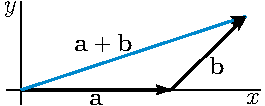
\includegraphics{add1.pdf}\qquad
     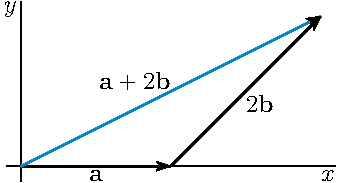
\includegraphics{add2.pdf}
\end{center}
\begin{center}
     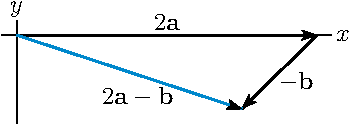
\includegraphics{add3.pdf}
\end{center}

\end{answer}

\begin{solution}
$\va+\vb=\llt 3,1\rgt $, $\va+2\vb=\llt 4,2\rgt $,\ 
$2\va-\vb=\llt 3,-1\rgt $

\begin{center}
     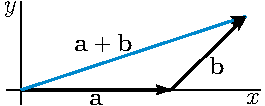
\includegraphics{add1.pdf}\qquad
     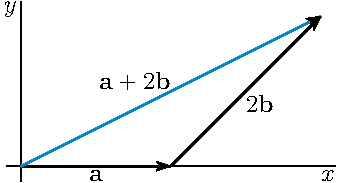
\includegraphics{add2.pdf}
\end{center}
\begin{center}
     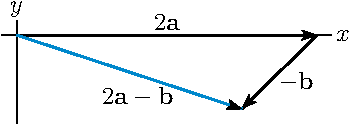
\includegraphics{add3.pdf}
\end{center}

\end{solution}

%%%%%%%%%%%%%%%%%%%%%%%%%%%%%%%%%%%%
\begin{question}
Determine whether or not the given points are collinear (that is, 
lie on a common straight line)
\begin{enumerate}[(a)]
\item
 $(1,2,3),\ (0,3,7),\ (3,5,11)$

\item
$(0,3,-5),\ (1,2,-2),\ (3,0,4)$
\end{enumerate}
\end{question}

\begin{hint}
If three points are collinear, then the vector from the first point
to the second point, and the vector from the first point to the third point 
must both be parallel to the line, and hence must be parallel to each other
(i.e. must be multiples of each other).

\begin{center}
     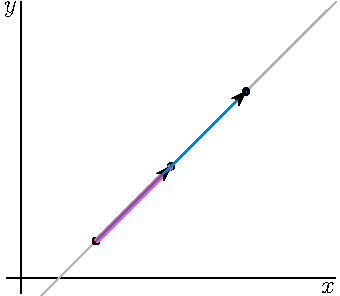
\includegraphics{collinear.pdf}
\end{center}

\end{hint}

\begin{answer}
(a) not collinear\qquad
(b) collinear
\end{answer}

\begin{solution}
If three points are collinear, then the vector from the first point
to the second point, and the vector from the first point to the third point 
must both be parallel to the line, and hence must be parallel to each other
(i.e. must be multiples of each other).

\begin{center}
     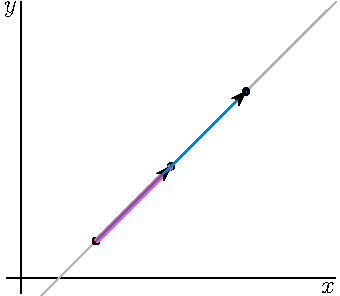
\includegraphics{collinear.pdf}
\end{center}

(a)
The vectors $\llt 0,3,7\rgt -\llt 1,2,3\rgt =\llt -1,1,4\rgt $ and $\llt 3,5,11\rgt -\llt 1,2,3\rgt =\llt 2,3,8\rgt $ 
are not parallel (i.e. are not multiples of each other),
so the three points are not on the same line.

(b)
The vectors $\llt 1,2,-2\rgt -\llt 0,3,-5\rgt =\llt 1,-1,3\rgt $ and
$\llt 3,0,4\rgt -\llt 0,3,-5\rgt =\llt 3,-3,9\rgt $ are parallel (i.e. are  multiples of each other),
so the three points are on the same line.
\end{solution}

%%%%%%%%%%%%%%%%%%%%%%%%%%%%%%%%
\begin{question}
Determine whether the given pair of vectors is perpendicular
\begin{enumerate}[(a)]
\item
$\llt 1,3,2\rgt ,\ \llt 2,-2,2\rgt $ 
\item
$\llt -3,1,7\rgt ,\ \llt 2,-1,1\rgt $ 
\item
$\llt 2,1,1\rgt ,\ \llt -1,4,2\rgt $ 
\end{enumerate}
\end{question}

\begin{hint}
Review Theorem \eref{CLP200}{thm:dotPppties} in the CLP-3 text.
\end{hint}

\begin{answer}
(a) perpendicular\qquad
(b) perpendicular\qquad
(c) not perpendicular
\end{answer}

\begin{solution}
\leqnomode
By property 7 of Theorem \eref{CLP200}{thm:dotPppties} in the CLP-3 text,
\begin{alignat*}{3}
\llt 1,3,2\rgt \cdot\llt 2,-2,2\rgt 
&=1\times2-3\times 2+2\times2=0\ 
&&\implies\ \text{perpendicular}
\tag{a} \\
\llt -3,1,7\rgt \cdot\llt 2,-1,1\rgt 
&=-3\times2-1\times 1+7\times1=0\ 
&&\implies\ \text{perpendicular}
\tag{b} \\
\llt 2,1,1\rgt \cdot\llt -1,4,2\rgt 
&=-2\times1+1\times 4+1\times2=4\ne 0\ 
&&\implies\ \text{not perpendicular}
\tag{c}
\end{alignat*}
\reqnomode
\end{solution}


%%%%%%%%%%%%%%%%%%%%%%%%%%%%%%%%
\begin{question}
Consider the vector $\va=\llt 3,4 \rgt$.
\begin{enumerate}[(a)]
\item
Find a unit vector in the same direction as $\va$. 
\item
Find all unit vectors that are parallel to $\va$.
\item
Find all vectors that are parallel to $\va$ and have length $10$.
\item
Find all unit vectors that are perpendicular to $\va$.
\end{enumerate}
\end{question}

\begin{hint}
Review Definition \eref{CLP200}{def parallel vectors} and 
Theorem \eref{CLP200}{thm:dotPppties} in the CLP-3 text.
\end{hint}

\begin{answer}
(a) $\frac{1}{5}\llt 3,4 \rgt$\quad
(b) $\pm\frac{1}{5}\llt 3,4 \rgt$\quad
(c) $\pm \llt 6,8 \rgt$\quad
(d) $\pm\frac{1}{5}\llt 4,-3 \rgt$
\end{answer}

\begin{solution}
(a) The vector $\va$ has length
\begin{equation*}
|\llt 3,4 \rgt|
=\sqrt{3^2+4^2}
=\sqrt{25}
=5
\end{equation*}
So the vector $\frac{1}{5}\llt 3,4 \rgt$ has length $1$ (i.e. is a unit vector)
and is in the same direction as  $\llt 3,4 \rgt$.

(b) Recall, from Definition \eref{CLP200}{def parallel vectors} in the CLP-3 text, that a vector is parallel to $\va$ if and only if it is of the form $s\va$
for some nonzero real number $s$. Such a vector is a unit vector if and only if
\begin{align*}
|s\va|=1
&\iff |s|\,|\llt 3,4 \rgt|=1
\iff |s| = \frac{1}{|\llt 3,4 \rgt|}= \frac{1}{5} \\
&\iff s  = \pm \frac{1}{5}
\end{align*}
So there are two unit vectors that are parallel to $\va$, namely
$\pm\frac{1}{5}\llt 3,4 \rgt$.

(c) We have already found, in part (b), all vectors that are parallel to $\va$ and have length $1$, namely $\pm\frac{1}{5}\llt 3,4 \rgt$. To increase the 
lengths of those vectors to $10$, we just need to multiply them by $10$, giving
$\pm\frac{10}{5}\llt 3,4 \rgt=\pm 2\llt 3,4 \rgt=\pm\llt 6,8 \rgt$.

(d) A vector $\llt x,y \rgt$ is perpendicular to $\va=\llt 3,4\rgt$
if and only if
\begin{equation*}
0=\llt x,y \rgt\cdot\llt 3,4\rgt
 = 3x+4y
\iff y=-\frac{3}{4}x
\iff \llt x,y \rgt = \llt x,-\frac{3}{4}x \rgt = \frac{x}{4} \llt 4,-3\rgt
\end{equation*}
 Such a vector is a unit vector if and only if
\begin{align*}
 \frac{|x|}{4}\,|\llt 4,-3 \rgt|=1
&\iff \frac{|x|}{4} = \frac{1}{|\llt 4,-3 \rgt|}= \frac{1}{5} \\
&\iff \frac{x}{4}   = \pm \frac{1}{5}
\end{align*}
So there are two unit vectors that are perpendicular to $\va$, namely
$\pm\frac{1}{5}\llt 4,-3 \rgt$.



\end{solution}


%%%%%%%%%%%%%%%%%%%%%%%%%%%%%%%%
\begin{question}
Consider the vector $\vb=\llt 3,4,0 \rgt$.
\begin{enumerate}[(a)]
\item
Find a unit vector in the same direction as $\vb$. 
\item
Find all unit vectors that are parallel to $\vb$.
\item
Find four different unit vectors that are perpendicular to $\vb$.
\end{enumerate}
\end{question}

\begin{hint}
Review Definition \eref{CLP200}{def parallel vectors} and 
Theorem \eref{CLP200}{thm:dotPppties} in the CLP-3 text.
\end{hint}

\begin{answer}
(a) $\frac{1}{5}\llt 3,4,0 \rgt$\quad
(b) $\pm\frac{1}{5}\llt 3,4,0 \rgt$

(c) A vector is of length one and perpendicular to $\vb$ if and only if it is of the form $\llt x,-\frac{3}{4}x,z \rgt $ with $\sqrt{\frac{25}{16}x^2+z^2}=1$.
There are infinitely many such vectors. Four of them are 
\begin{equation*}
\pm\llt 0,0,1\rgt\qquad
\pm\frac{1}{5}\llt 4,-3,0\rgt
\end{equation*}

\end{answer}

\begin{solution}
(a) The vector $\vb$ has length
\begin{equation*}
|\llt 3,4,0 \rgt|
=\sqrt{3^2+4^2+0^2}
=\sqrt{25}
=5
\end{equation*}
So the vector $\frac{1}{5}\llt 3,4,0 \rgt$ has length $1$ (i.e. is a 
unit vector) and is in the same direction as  $\llt 3,4,0 \rgt$.

(b) Recall, from Definition \eref{CLP200}{def parallel vectors} in the CLP-3 text, that a vector is parallel to $\vb$ if and only if it is of the form $s\vb$
for some nonzero real number $s$. Such a vector is a unit vector if and only if
\begin{align*}
|s\vb|=1
&\iff |s|\,|\llt 3,4,0 \rgt|=1
\iff |s| = \frac{1}{|\llt 3,4,0 \rgt|}= \frac{1}{5} \\
&\iff s  = \pm \frac{1}{5}
\end{align*}
So there are two unit vectors that are parallel to $\vb$, namely
$\pm\frac{1}{5}\llt 3,4,0 \rgt$.

(c) A vector $\llt x,y,z \rgt$ is perpendicular to $\va=\llt 3,4,0\rgt$
if and only if
\begin{equation*}
0=\llt x,y,z \rgt\cdot\llt 3,4,0\rgt
 = 3x+4y
\iff y=-\frac{3}{4}x
\iff \llt x,y,z \rgt = \llt x,-\frac{3}{4}x,z \rgt 
\end{equation*}
 Such a vector is a unit vector if and only if
\begin{align*}
 \left|\llt x,-\frac{3}{4}x,z \rgt\right|=1
&\iff \sqrt{x^2+\frac{9}{16}x^2+z^2}=1
 \iff \sqrt{\frac{25}{16}x^2+z^2}=1
\end{align*}
There are infinitely many pairs $x$, $z$ that 
obey $\sqrt{\frac{25}{16}x^2+z^2}=1$. We can easily get two of them
by setting $x=0$ and choosing $z$ to obey $\sqrt{z^2}=1$, i.e. choosing 
$z=\pm 1$. We can easily get two more of them
by setting $z=0$ and choosing $x$ to obey $\sqrt{\frac{25}{16}x^2}=1$, 
i.e. choosing $x=\pm \frac{4}{5}$. This gives us four vectors of length one that
are perpendicular to $\vb$, namely
\begin{equation*}
\pm\llt 0,0,1\rgt\qquad
\pm\llt \frac{4}{5}\,,\,-\frac{3}{4}\,\frac{4}{5}\,,\,0\rgt
=\pm\frac{1}{5}\llt 4,-3,0\rgt
\end{equation*}

\end{solution}



%%%%%%%%%%%%%%%%%%%%%%%%%%%%%%%%%%%%
\begin{question}
Let $\va=\llt a_1,a_2\rgt$. Compute the projection of $\va$ on
$\hi$ and $\hj$.
\end{question}

%\begin{hint}
%\end{hint}

\begin{answer}
$\text{proj}_{\hi}\va=a_1\hi$\qquad
$\text{proj}_{\hj}\va=a_2\hj$.
\end{answer}

\begin{solution}
$\text{proj}_{\hi}\va=(\va\cdot\hi)\hi
=a_1\hi$ and
$\text{proj}_{\hj}\va=(\va\cdot\hj)\hj
=a_2\hj$.
\end{solution}

%%%%%%%%%%%%%%%%%%%%%%%%%%%%%%%%%%%%
\begin{question}
Does the triangle with vertices $(1,2,3),\ (4,0,5)$ and $(3,6,4)$
have a right angle?
\end{question}

%\begin{hint}
%\end{hint}

\begin{answer}
Yes.
\end{answer}

\begin{solution}
The vector from $(1,2,3)$ to $(4,0,5)$ is $\llt 3,-2,2\rgt$.
The vector from $(1,2,3)$ to $(3,6,4)$ is $\llt 2,4,1\rgt$.
The dot product between these two vectors is 
$\llt 3,-2,2\rgt\cdot\llt 2,4,1\rgt=0$,
so the vectors are perpendicular and the triangle does contain a right
angle.

\end{solution}

%%%%%%%%%%%%%%%%%%%%%%%%%%%%%
\begin{question}
Show that the area of the parallelogram determined by the
vectors $\va$ and $\vb$ is $|\va\times \vb|$.

\begin{center}
     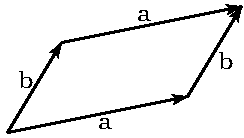
\includegraphics{sec_1_2_pgramA.pdf}
\end{center}

\end{question}

%\begin{hint}
%\end{hint}

\begin{answer}
See the solution.
\end{answer}

\begin{solution}
 The area of a parallelogram is the length of its
base time its height. 
\vadjust{
\begin{center}
     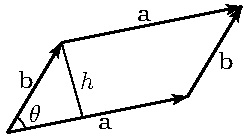
\includegraphics{sec_1_2_pgramB.pdf}
\end{center}
}%
We can choose the base to be $\va$. Then, if $\theta$
is the angle between its sides $\va$ and $\vb$, its height is 
$|\vb|\sin\theta$.  
So
\begin{equation*}
\text{area} = |\va||\vb|\sin\theta=|\va\times\vb|
\end{equation*}
\end{solution}

%%%%%%%%%%%%%%%%%%%%%%%%%%%%%
\begin{question}
Show that the volume of the parallelepiped determined by the
vectors $\va,\ \vb$ and $\vc$ is 
\begin{equation*}
    |\va\cdot(\vb\times\vc)|
\end{equation*}

\begin{center}
     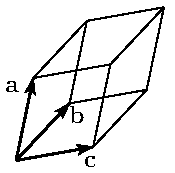
\includegraphics{piped.pdf}
\end{center}

\end{question}

%\begin{hint}
%\end{hint}

\begin{answer}
See the solution
\end{answer}

\begin{solution}
The volume of a parallelepiped is the area of its
base time its height. We can choose the base to be the parallelogram 
determined by the vectors $\vb$ and $\vc$. It has area $|\vb\times\vc|$.
The vector $\vb\times\vc$ is perpendicular to the base. 
\vadjust{
\begin{center}
     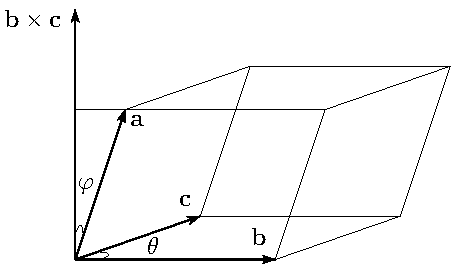
\includegraphics{pipedVolume.pdf}
\end{center}
}%
Denote by
$\theta$ the angle between $\va$ and the perpendicular $\vb\times\vc$.
The height of the parallelepiped is $|\va| |\cos\theta|$. So 
\begin{equation*}
\text{volume} = |\va|\, |\cos\theta|\, |\vb\times\vc|
=|\va\cdot(\vb\times\vc)|
\end{equation*}
\end{solution}

%%%%%%%%%%%%%%%%%%%%%%%%%%%%%%%%
\begin{question}
Verify by direct computation that
\begin{enumerate}[(a)]
\item
$\hi\times\hj=\hk$, $\hj\times\hk=\hi$, $\hk\times\hi=\hj$
\item
$\va\cdot(\va\times\vb)=\vb\cdot(\va\times\vb)=\vZero$
\end{enumerate}
\end{question}

%\begin{hint}
%
%\end{hint}

\begin{answer}
See the solution.
\end{answer}

\begin{solution}
(a)
\begin{alignat*}{5}
\hi\times\hj&=\det\left[\begin{matrix}\hi&\hj &\hk\\
                     1&0&0\\
                     0&1&0\end{matrix}\right]
&&=\hi(0\times 0-0\times 1)
-\hj(1\times 0-0\times 0)
+\hk(1\times 1-0\times 0) \\
&=\hk\\[0.1in]
%%
\hj\times\hk&=\det\left[\begin{matrix}\hi&\hj &\hk\\
                     0&1&0\\
                     0&0&1\end{matrix}\right]
&&=\hi(1\times 1-0\times 0)
-\hj(0\times 1-0\times 0)
+\hk(0\times 0-1\times 0)\\
&=\hi\\[0.1in]
%%
\hk\times\hi&=\det\left[\begin{matrix}\hi&\hj &\hk\\
                     0&0&1\\
                     1&0&0\end{matrix}\right]
&&=\hi(0\times 0-1\times 0)
-\hj(0\times 0-1\times 1)
+\hk(0\times 0-0\times 1)\\
&=\hj
\end{alignat*}

(b)
\begin{alignat*}{5}
\va\cdot(\va\times\vb)
&=a_1\big(a_2b_3-a_3b_2\big)
  -a_2\big(a_1b_3-a_3b_1\big)
  +a_3\big(a_1b_2-a_2b_1\big)
&&=0\\
\vb\cdot(\va\times\vb)
&=b_1\big(a_2b_3-a_3b_2\big)
  -b_2\big(a_1b_3-a_3b_1\big)
  +b_3\big(a_1b_2-a_2b_1\big)
&&=0
\end{alignat*}
\end{solution}




%%%%%%%%%%%%%%%%%%%%%%%%%%%%%%%%
\begin{question}
Consider the following statement: ``If $\va\ne\vZero$
and if $\va\cdot\vb=\va\cdot\vc$ then $\vb=\vc$.''
If the statment is true, prove it. If the statement is false, give a 
counterexample.
\end{question}

%\begin{hint}
%
%\end{hint}

\begin{answer}
This statement is false. One counterexample is $\va=\llt 1,0,0\rgt $,
$\vb=\llt 0,1,0\rgt ,\ \vc=\llt 0,0,1\rgt $. Then $\va\cdot\vb=\va\cdot\vc=0$, but $\vb\ne\vc$. There are \emph{many} other counterexamples.
\end{answer}

\begin{solution}
This statement is false. The two numbers 
$\va\cdot\vb$, $\va\cdot\vc$ are equal if and only if
$\va\cdot(\vb-\vc)= 0$. This in turn is the case if and only
if $\va$ is perpendicular to $\vb-\vc$ (under the convention that
$\vZero$ is perpendicular to all vectors). For example, 
if $\va=\llt 1,0,0\rgt $, $\vb=\llt 0,1,0\rgt ,\ \vc=\llt 0,0,1\rgt $, then $\vb-\vc=\llt 0,1,-1\rgt$ is perpendicular to $\va$ so that 
$\va\cdot\vb=\va\cdot\vc$.
\end{solution}

%%%%%%%%%%%%%%%%%%%%%%%%%%%%%%%%%%%%
\begin{question}\label{PRB Qnine}
Consider the following statement: ``The vector $\va\times(\vb\times\vc)$ 
is of the form $\al\vb+\be\vc$ for some real numbers $\al$ and $\be$.''
If the statement is true, prove it. If the statement is false, give a 
counterexample.

\end{question}

%\begin{hint}
%\end{hint}

\begin{answer}
True.
\end{answer}

\begin{solution}
This statement is true. In the event that $\vb$ and 
$\vc$ are parallel, $\vb\times\vc=\vZero$ so that
$\va\times(\vb\times\vc)=\vZero=0\vb+0\vc$, so we may assume
that $\vb$ and $\vc$ are not parallel. Then as $\al$ and $\be$ run
over $\bbbr$, the vector $\al\vb+\be \vc$ runs over the plane that
contains the origin and the vectors $\vb$ and $\vc$. Call this plane
$P$. Because
$\vd=\vb\times\vc$ is nonzero and perpendicular to both 
$\vb$ and $\vc$, $P$ is the plane that contains the origin
and is perpendicular to $\vd$. As $\va\times(\vb\times\vc)=\va\times\vd$ is always perpendicular to $\vd$, it lies in $P$.
\end{solution}

%%%%%%%%%%%%%%%%%%%%%%%%%%%%%%%%%%%%
\begin{question}
What geometric conclusions can you draw from
$\va\cdot(\vb\times\vc)=\llt 1,2,3\rgt$?
\end{question}

%\begin{hint}
%\end{hint}

\begin{answer}
None. The given equation is nonsense.
\end{answer}

\begin{solution}
None. The given equation is nonsense. The left hand side is
a number while the right hand side is a vector.
\end{solution}

%%%%%%%%%%%%%%%%%%%%%%%%%%%%%%%%%%%%
\begin{question}
What geometric conclusions can you draw from
$\va\cdot(\vb\times\vc)=0$?
\end{question}

%\begin{hint}
%\end{hint}

\begin{answer}
If $\vb$ and $\vc$ are parallel, then $\va\cdot(\vb\times\vc)=0$ for all $\va$.
If $\vb$ and $\vc$ are not parallel, then $\va$ must be of the form  
$\al\vb+\be\vc$ with $\al$ and $\be$ real numbers.
\end{answer}

\begin{solution}
If $\vb$ and $\vc$ are parallel, then $\vb\times\vc=\vZero$
and $\va\cdot(\vb\times\vc)=0$ for all $\va$.
If $\vb$ and $\vc$ are not parallel, $\va\cdot(\vb\times\vc)=0$ 
if and only if $\va$ is perpendicular to $\vd=\vb\times\vc$.
As we saw in question \ref{PRB Qnine}, the set of all vectors perpendicular to
$\vd$ is the plane consisting of all vectors of the form  
$\al\vb+\be\vc$ with $\al$ and $\be$ real numbers. So $\va$ must
be of this form.
\end{solution}

%%%%%%%%%%%%%%%%%%%%%%%%%%%%%%%%%%%%
\begin{question}
Consider the three points $O=(0,0)$, $A=(a,0)$ and $B=(b,c)$.
\begin{enumerate}[(a)]
\item
Sketch, in a single figure,
\begin{itemize}\itemsep1pt \parskip0pt \parsep0pt %\itemindent-15pt
\item
the triangle with vertices $O$, $A$ and $B$, and
\item
the circumscribing circle for the triangle (i.e. the circle that goes 
through all three vertices), and
\item
the vectors
\begin{itemize}\itemsep1pt \parskip0pt \parsep0pt %\itemindent-15pt
\item 
$\overrightarrow{OA}$, from $O$ to $A$,
\item 
$\overrightarrow{OB}$, from $O$ to $B$,
\item 
$\overrightarrow{OC}$, from $O$ to $C$, where $C$ is the centre of the circumscribing circle.
\end{itemize}
\end{itemize}
Then add to the sketch and evaluate, from the sketch,
\begin{itemize}\itemsep1pt \parskip0pt \parsep0pt %\itemindent-15pt
\item 
the projection of the vector $\overrightarrow{OC}$ on the vector 
$\overrightarrow{OA}$, and
\item 
the projection of the vector $\overrightarrow{OC}$ on the vector 
$\overrightarrow{OB}$.
\end{itemize}

\item Determine $C$.

\item
Evaluate, using the formula (\eref{CLP200}{eqn proj}) in the CLP-3 text,
\begin{itemize}\itemsep1pt \parskip0pt \parsep0pt %\itemindent-15pt
\item 
the projection of the vector $\overrightarrow{OC}$ on the vector 
$\overrightarrow{OA}$, and
\item 
the projection of the vector $\overrightarrow{OC}$ on the vector 
$\overrightarrow{OB}$.
\end{itemize}
\end{enumerate}
\end{question}

\begin{hint}
(a)
The three line segments from $C$ to $O$, from $C$ to $A$ and from $C$ to $B$
all have exactly the same length, namely the radius of the circumscribing 
circle.

(b) 
Let $(\bar x,\bar y)$ be the coordinates of $C$.
Write down the equations that say that $(\bar x,\bar y)$ is
equidistant from the three vertices $O$, $A$ and $B$.
\end{hint}

\begin{answer}
(a), (c)
\begin{center}
     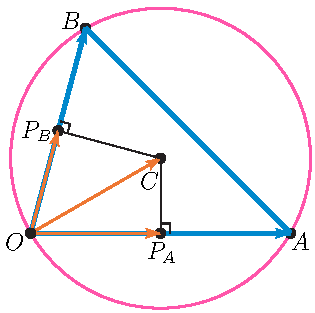
\includegraphics{circumA.pdf}
\end{center}
$\text{proj}_{\overrightarrow{\scriptstyle OA}}\,\overrightarrow{OC}
    =\overrightarrow{OP_A}=\llt a/2,0\rgt$\qquad
$\text{proj}_{\overrightarrow{\scriptstyle OB}}\,\overrightarrow{OC}
    =\overrightarrow{OP_A}=\llt b/2,c/2\rgt$

(b) The centre of the circumscribing circle is $(\bar x,\bar y)$ with
$\bar x=\frac{a}{2}$ and
$ \bar y =\frac{b^2+c^2-ab}{2c}$.
\end{answer}

\begin{solution}
(a) The sketch for part (a) is on the left below.
To sketch the projections, we dropped perpendiculars 
\begin{itemize}\itemsep1pt \parskip0pt \parsep0pt %\itemindent-15pt
\item 
from $C$ to the line from $O$ to $A$, and 
\item 
from $C$ to the line from $O$ to $B$.
\end{itemize}
By definition, 
\begin{itemize}\itemsep1pt \parskip0pt \parsep0pt %\itemindent-15pt
\item 
$\text{proj}_{\overrightarrow{\scriptstyle OA}}\,\overrightarrow{OC}$
is the vector $\overrightarrow{OP_A}$ from $O$ to the point $P_A$, where 
the perpendicular from $C$ to the line from $O$ to $A$ hits the line,
and 
\item 
$\text{proj}_{\overrightarrow{\scriptstyle OB}}\,\overrightarrow{OC}$
is the vector $\overrightarrow{OP_B}$ from $O$ to the point $P_B$, where 
the perpendicular from $C$ to the line from $O$ to $B$ hits the line.
\end{itemize}
\begin{center}
     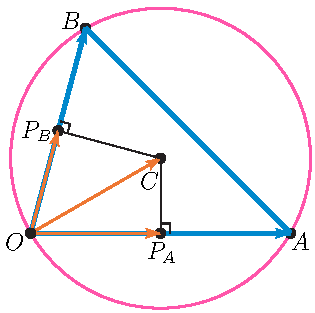
\includegraphics{circumA.pdf}\qquad\qquad
     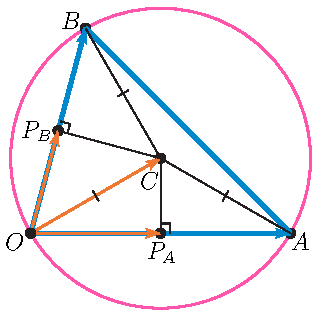
\includegraphics{circum.pdf}
\end{center}
To evaluate the projections we observe that the three lines from 
$C$ to $O$, from $C$ to $A$ and from $C$ to $B$ all have exactly the same length
(namely the radius of the circumscribing circle). Consequently
(see the figure on the right above),
\begin{itemize}\itemsep1pt \parskip0pt \parsep0pt %\itemindent-15pt
\item 
the triangle $OCA$ is an isoceles triangle, so that $P_A$ is exactly the
midpoint of the line segement from $O$ to $A$. That is, $P_A$ is $(a/2,0)$ and
\begin{equation*}
\text{proj}_{\overrightarrow{\scriptstyle OA}}\,\overrightarrow{OC}
    =\overrightarrow{OP_A}=\llt a/2,0\rgt
\end{equation*}
\item 
Similarly, the triangle $OCB$ is an isoceles triangle, so that $P_B$ is 
exactly the midpoint of the line segement from $O$ to $B$. That is $P_A$ is $(b/2,c/2)$ and
\begin{equation*}
\text{proj}_{\overrightarrow{\scriptstyle OB}}\,\overrightarrow{OC}
    =\overrightarrow{OP_B}=\llt b/2,c/2\rgt
\end{equation*}
\end{itemize}

(b)
Call the centre of the circumscribing circle $(\bar x,\bar y)$. 
This centre must be equidistant from the three vertices.
So
\begin{align*}
\bar x^2+\bar y^2=(\bar x-a)^2+\bar y^2=(\bar x-b)^2+(\bar y-c)^2 
\end{align*}
or, subtracting $\bar x^2+\bar y^2$ from all three expression,
\begin{align*}
0=a^2-2a\bar x=b^2-2b\bar x+c^2-2c\bar y
\end{align*}
which implies
\begin{equation*}
\bar x=\frac{a}{2}\qquad\qquad \bar y
=\frac{b^2+c^2-2b\bar x}{2c}=\frac{b^2+c^2-ab}{2c}
\end{equation*}


(c) From part (b), we have
\begin{align*}
\overrightarrow{OA}\cdot\overrightarrow{OC}
&=\llt a,0\rgt\cdot\llt\frac{a}{2}\,,\,\frac{b^2+c^2-ab}{2c}\rgt
=\frac{a^2}{2}=\frac{1}{2}|\overrightarrow{OA}|^2\\
\overrightarrow{OB}\cdot\overrightarrow{OC}
&=\llt b,c\rgt\cdot\llt\frac{a}{2}\,,\,\frac{b^2+c^2-ab}{2c}\rgt
=\frac{ab}{2}+\frac{b^2+c^2-ab}{2}=\frac{b^2+c^2}{2}
=\frac{1}{2}|\overrightarrow{OB}|^2 
\end{align*}
So, by Equation (\eref{CLP200}{eqn proj}) in the CLP-3 text,
\begin{align*}
\text{proj}_{\overrightarrow{\scriptstyle OA}}\,\overrightarrow{OC}
&=\frac{\overrightarrow{OA}\cdot\overrightarrow{OC}}{|\overrightarrow{OA}|^2}
           \overrightarrow{OA}
=\frac{1}{2}\overrightarrow{OA}
=\llt a/2,0\rgt \\
\text{proj}_{\overrightarrow{\scriptstyle OB}}\,\overrightarrow{OC}
&=\frac{\overrightarrow{OB}\cdot\overrightarrow{OC}}{|\overrightarrow{OB}|^2}
           \overrightarrow{OB}
=\frac{1}{2}\overrightarrow{OB}
=\llt b/2,c/2\rgt
\end{align*}


\end{solution}






%%%%%%%%%%%%%%%%%%%%%%%%%%%%
%\Instructions{Questions~\ref{prob_s1.0first} through \ref{prob_s1.0last} provide practice with.}
%%%%%%%%%%%%%%%%%%%%

%%%%%%%%%%%%%%%%%%
\subsection*{\Procedural}
%%%%%%%%%%%%%%%%%%

%%%%%%%%%%%%%%%%%%%%%%%%%%%%%%%%%%%%
\begin{question}
Find the equation of a sphere if one of its diameters has end
points $(2,1,4)$ and $(4,3,10)$.
\end{question}

\begin{hint}
The centre of the sphere is the midpoint of the diameter.
\end{hint}

\begin{answer}
$(x-3)^2+(y-2)^2+(z-7)^2=11$
\end{answer}

\begin{solution}
The center of the sphere is 
$\half\big\{(2,1,4)+(4,3,10)\big\}=(3,2,7)$. The diameter (i.e. twice the radius) is $|(2,1,4)-(4,3,10)|=|(-2,-2,-6)|=2|(1,1,3)|=2\sqrt{11}$. So the radius of the sphere is $\sqrt{11}$ and
the equation of the sphere is
\begin{equation*}
(x-3)^2+(y-2)^2+(z-7)^2=11
\end{equation*}
\end{solution}


%%%%%%%%%%%%%%%%%%%%%%%%%%%%%%%%%%%%
\begin{question}
Use vectors to prove that the line joining the midpoints of two sides
of a triangle is parallel to the third side  and half its length.
\end{question}

\begin{hint}
Draw a sketch.
Call the vertices of the triangle $A$, $B$ and $C$ with $C$ being the
vertex that joins the two sides. Let $\va$ be the vector from $C$ to $A$ 
and $\vb$ be the vector from $C$ to $B$. Determine, in terms of $\va$ and 
$\vb$, 
\begin{itemize}\itemsep0pt \parskip0pt \parsep0pt %\itemindent-15pt

\item 
the vector from $A$ to $B$, 
\item
the two vectors from $C$ to the two midpoints and finally 
\item
the vector joining the two midpoints. 
\end{itemize}
\end{hint}

\begin{answer}
See the solution.
\end{answer}

\begin{solution}
Call the vertices of the triangle $A$, $B$ and $C$ with $C$ being the
vertex that joins the two sides. We can always
choose our coordinate system so that $C$ is at the origin.
Let $\va$ be the vector from $C$ to $A$ 
and $\vb$ be the vector from $C$ to $B$.
\begin{center}
     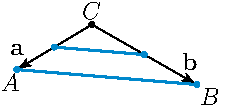
\includegraphics{triangleMidPt.pdf}
\end{center}
\begin{itemize}
\item
Then the vector from $C$ to the midpoint of the side from $C$ to $A$ is
$\half\va$ and
\item
the vector from $C$ to the midpoint of the side from $C$ to $B$ is
$\half\vb$ so that
\item
the vector joining the two midpoints is $\half\vb-\half\va$. 
\end{itemize}
As the vector from $A$ to $B$ is $\vb-\va=2\big[\half\vb-\half\va\big]$,
the line joining the midpoints is indeed parallel to the third side
and half its length.
\end{solution}


%%%%%%%%%%%%%%%%%%%%%%%%%%%%%%%%
\begin{question}
Compute the areas of the parallelograms determined by the
following vectors.
\begin{enumerate}[(a)]
\item
$\llt -3,1\rgt,\ \llt 4,3\rgt$ 
\item
$\llt 4,2\rgt,\ \llt 6,8\rgt$
\end{enumerate}
\end{question}

\begin{hint}
Review \S\eref{CLP200}{sec:GEOparallelogram} in the CLP-3 text.
\end{hint}

\begin{answer}
(a) $13$\qquad
(b) $20$
\end{answer}

\begin{solution} (a)
By (\eref{CLP200}{eq pgram area}) in the CLP-3 text, the area is 
\begin{align*}
\left| \det\left[\begin{matrix}-3&1 \\ 4&3 \end{matrix}\right] \right|
  &=\big|-3\times 3-1\times 4\big| = |-13| = 13
\end{align*}

(b)
By (\eref{CLP200}{eq pgram area}) in the CLP-3 text, the area is 
\begin{align*}
\left|\det\left[\begin{matrix} 4&2 \\ 6&8 \end{matrix}\right]\right| 
&=\big|4\times 8-2\times 6\big| 
= 20
\end{align*}
\end{solution}

\begin{question}[M200 2014A] %1c
Consider the plane $W$, defined by:
\begin{equation*}
W\ :\ -x + 3y + 3z = 6,\qquad
\end{equation*}
Find the area of the parallelogram on $W$ defined by 
$0 \le x \le 3$, $0 \le y \le 2$.
\end{question}

\begin{hint}
Determine the four corners of the parallelogram.
\end{hint}

\begin{answer}
$2\sqrt{19}$
\end{answer}

\begin{solution}
Note that 
\begin{itemize}
   \item the point on $W$ with $x=0$, $y=0$ obeys 
                         $-0+3(0)+3z=6$ and so has $z=2$
   \item the point on $W$ with $x=0$, $y=2$ obeys 
                         $-0+3(2)+3z=6$ and so has $z=0$
   \item the point on $W$ with $x=3$, $y=0$ obeys 
                         $-3+3(0)+3z=6$ and so has $z=3$
   \item the point on $W$ with $x=3$, $y=2$ obeys 
                         $-3+3(2)+3z=6$ and so has $z=1$
\end{itemize}
So the four corners of the parallelogram are 
$(0,0,2)$, $(0,2,0)$, $(3,0,3)$ and $(3,2,1)$. The vectors
\begin{align*}
\vd_1&=\llt 0-0 \,,\, 2-0 \,,\, 0-2 \rgt = \llt 0 \,,\, 2 \,,\, -2\rgt \\
\vd_2&=\llt 3-0 \,,\, 0-0 \,,\, 3-2 \rgt = \llt 3 \,,\, 0 \,,\, 1\rgt 
\end{align*}
form two sides of the paralleogram. So the area of the parallelogram is
\begin{align*}
\big|\vd_1\times\vd_2\big| 
=\left|\det\left[\begin{matrix}
                     \hi & \hj & \hk \\
                     0   &  2  & -2 \\
                     3   &  0  &  1
                \end{matrix}\right]\right|
=\left| 2\,\hi - 6\,\hj -6\hk  \right|
=\sqrt{76}
=2\sqrt{19}
\end{align*}

\end{solution}

%%%%%%%%%%%%%%%%%%%%%%%%%%%%%%%%
\begin{question}
Compute the volumes of the parallelepipeds determined by the
following vectors.
\begin{enumerate}[(a)]
\item
 $\llt 4,1,-1\rgt,\ \llt -1,5,2\rgt,\ \llt 1,1,6\rgt$ 
\item
  $\llt -2,1,2\rgt,\ \llt 3,1,2\rgt,\ \llt 0,2,5\rgt$
\end{enumerate}
\end{question}

\begin{hint}
Review \S\eref{CLP200}{sec:GEOparallelogram} in the CLP-3 text.
\end{hint}

\begin{answer}
(a) $126$\qquad
(b) $5$
\end{answer}

\begin{solution}
(a) 
By (\eref{CLP200}{eq piped volume}) in the CLP-3 text, the volume is 
\begin{align*}
\left| \det\left[\begin{matrix}
          4&1&-1 \\
         -1&5&2 \\
          1&1&6\end{matrix}\right] \right|
&=\left| 4\det\left[\begin{matrix}
          5&2 \\
          1&6 \end{matrix}\right]
        -1\det\left[\begin{matrix}
         -1&2 \\ 
          1&6 \end{matrix}\right]
        +(-1)\det\left[\begin{matrix}
         -1&5\\1&1\end{matrix}\right]\right| \\
&= \big|4(30-2)-1(-6-2)-1(-1-5)\big| = 4\times28+8+6\\
&=126
\end{align*}

(b)
By (\eref{CLP200}{eq piped volume}) in the CLP-3 text, the volume is 
\begin{align*}
\left|\det\left[\begin{matrix}
       -2&1&2\\
       3&1&2\\
       0&2&5\end{matrix}\right] \right|
&=\left|-2\det\left[\begin{matrix}
          1&2\\
          2&5\end{matrix}\right]
        -1\det\left[\begin{matrix}
          3&2\\
          0&5\end{matrix}\right]
       +2\det\left[\begin{matrix}
         3&1\\
         0&2\end{matrix}\right] \right|\\
&=\big|-2(5-4)-1(15-0)+2(6-0)\big| =\big|-2-15+12\big|=\big|-5\big|\\
&=5
\end{align*}
\end{solution}

%%%%%%%%%%%%%%%%%%%%%%%%%%%%%%%%%%%%
\begin{question}
Compute the dot product of the vectors $\va$ and $\vb$.
Find the angle between them.
\begin{enumerate}[(a)]
\item $\va=\llt 1,2\rgt ,\ \vb=\llt -2,3\rgt $
\item $\va=\llt -1,1\rgt ,\ \vb=\llt 1,1\rgt $
\item $\va=\llt 1,1\rgt ,\ \vb=\llt 2,2\rgt $
\item $\va=\llt 1,2,1\rgt ,\ \vb=\llt -1,1,1\rgt $
\item $\va=\llt -1,2,3\rgt ,\ \vb=\llt 3,0,1\rgt $
\end{enumerate}
\end{question}

%\begin{hint}
%\end{hint}

\begin{answer}
\leqnomode
\begin{alignat*}{3}
\va\cdot\vb&=4\qquad &
\theta &= 60.25^\circ\hskip4in 
\tag{a}\\
\va\cdot\vb&=0 &
\theta &= 90^\circ 
\tag{b}\\
\va\cdot\vb&=4 &
\theta &= 0^\circ 
\tag{c}\\
\va\cdot\vb&=2 &
\theta &= 61.87^\circ 
\tag{d}\\
\va\cdot\vb&=0 &
\theta &= 90^\circ 
\tag{e}
\end{alignat*}
\reqnomode
\end{answer}

\begin{solution}
\leqnomode
\begin{align*}
\va\cdot\vb&=\llt 1,2\rgt\cdot\llt -2,3\rgt=4 &
\cos\theta&=\frac{4}{\sqrt{5}\sqrt{13}}=.4961 &
\theta &= 60.25^\circ 
\tag{a}\\
\va\cdot\vb&=\llt -1,1\rgt\cdot\llt 1,1\rgt=0 &
\cos\theta&=\frac{0}{\sqrt{2}\sqrt{2}}=0 &
\theta &= 90^\circ 
\tag{b}\\
\va\cdot\vb&=\llt 1,1\rgt\cdot\llt 2,2\rgt=4 &
\cos\theta&=\frac{4}{\sqrt{2}\sqrt{8}}=1 &
\theta &= 0^\circ 
\tag{c}\\
\va\cdot\vb&=\llt 1,2,1\rgt\cdot\llt -1,1,1\rgt=2 &
\cos\theta&=\frac{2}{\sqrt{6}\sqrt{3}}=.4714 &
\theta &= 61.87^\circ 
\tag{d}\\
\va\cdot\vb&=\llt -1,2,3\rgt\cdot\llt 3,0,1\rgt=0 &
\cos\theta&=\frac{0}{\sqrt{14}\sqrt{10}}=0 &
\theta &= 90^\circ 
\tag{e}
\end{align*}
\reqnomode
\end{solution}

%%%%%%%%%%%%%%%%%%%%%%%%%%%%%%%%
\begin{question}
Determine the angle between the vectors $\va$ and $\vb$ if
\begin{enumerate}[(a)]
\item
   $\va=\llt 1,2\rgt,\ \vb=\llt 3,4\rgt$ 
\item
   $\va=\llt 2,1,4\rgt,\ \vb=\llt 4,-2,1\rgt$ 
\item
  $\va=\llt 1,-2,1\rgt,\ \vb=\llt 3,1,0\rgt$ 
\end{enumerate}
\end{question}

%\begin{hint}
%
%\end{hint}

\begin{answer}
(a) $10.3^\circ$\qquad
(b) $61.6^\circ$\qquad
(c) $82.6^\circ$
\end{answer}

\begin{solution}
\leqnomode
By property 6 of Theorem \eref{CLP200}{thm:dotPppties} in the CLP-3 text,
\begin{alignat*}{3}
&\cos\theta=\frac{\va\cdot\vb}{|\va|\,|\vb|}
        =\frac{1\times 3+2\times 4}{\sqrt{1+4}\sqrt{9+16}}
        =\frac{11}{5\sqrt{5}}= .9839 
\qquad &&\implies\quad \theta=10.3^\circ
\tag{a} \\
&\cos\theta=\frac{\va\cdot\vb}{|\va|\,|\vb|}
        =\frac{2\times 4-1\times 2+4\times 1}{\sqrt{4+1+16}\sqrt{16+4+1}}
        =\frac{10}{21}= .4762 
\qquad &&\implies\quad \theta=61.6^\circ
\tag{b} \\
 &\cos\theta=\frac{\va\cdot\vb}{|\va|\,|\vb|}
        =\frac{1\times 3-2\times 1+1\times 0}{\sqrt{1+4+1}\sqrt{9+1}}
        =\frac{1}{\sqrt{60}}= .1291 
\qquad &&\implies\quad \theta=82.6^\circ
\tag{c}
\end{alignat*}
\reqnomode
\end{solution}

%%%%%%%%%%%%%%%%%%%%%%%%%%%%%%%%
\begin{question}
Determine all values of $y$ for which the given vectors are perpendicular.
\begin{enumerate}[(a)]
\item
$\llt 2,4\rgt ,\ \llt 2,y\rgt $ 
\item
$\llt 4,-1\rgt ,\ \llt y,y^2\rgt $ 
\item
$\llt 3,1,1\rgt ,\ \llt 2,5y,y^2\rgt $ 
\end{enumerate}
\end{question}

%\begin{hint}
%
%\end{hint}

\begin{answer}
(a) $-1$\qquad
(b) $0$, $4$\qquad
(c) $-2$, $-3$
\end{answer}

\begin{solution}
\leqnomode
\begin{alignat*}{3}
&\llt 2,4\rgt \cdot\llt 2,y\rgt =2\times2+4\times y=4+4y=0
   &&\ \iff\  y=-1
\tag{a} \\
&\llt 4,-1\rgt \cdot\llt y,y^2\rgt =4\times y-1\times y^2=4y-y^2=0
   &&\ \iff\  y=0,4
\tag{b} \\
&\llt 3,1,1\rgt \cdot\llt 2,5y,y^2\rgt 
  %=3\times2+1\times 5y+1\times y^2
  =6+5y+y^2=0
   &&\ \iff\  y=-2,-3
\tag{c}
\end{alignat*}
\reqnomode
\end{solution}

%%%%%%%%%%%%%%%%%%%%%%%%%%%%%%%%
\begin{question}
Let $\vu=-2\hi+5\hj$ and $\vv=\al\hi-2\hj$. Find $\al$ so that
\begin{enumerate}[(a)]
\item
   $\vu\perp\vv$
\item
   $\vu \| \vv$
\item
   The angle between $\vu$ and $\vv$ is $60^\circ$.
\end{enumerate}
\end{question}

%\begin{hint}
%
%\end{hint}

\begin{answer}
(a) $-5$\qquad
(b) $0.8$\qquad
(c) none
\end{answer}

\begin{solution}
(a) 
   We want $0=\vu\cdot\vv=-2\al-10$ or $\al=-5$.

(b) 
   We want $-2/\al=5/(-2)$ or $\al=0.8$.

(c) 
   We want $\vu\cdot\vv=-2\al-10
             =|\vu|\,|\vv|\,\cos 60^\circ
             =\sqrt{29}\,\sqrt{\al^2+4}\,\half$. Squaring both sides gives
\begin{alignat*}{3}
& & 4\al^2+40\al+100&=\frac{29}{4}(\al^2+4) \\
&\implies\quad &  13\al^2-160\al-284&=0 \\
&\implies\quad & \al &=\frac{160\pm\sqrt{160^2+4\times13\times284}}{26}
\approx 13.88\text{ or }-1.574
\end{alignat*}
Both of these $\al$'s give $\vu\cdot\vv<0$ so no $\al$ works.
\end{solution}

%%%%%%%%%%%%%%%%%%%%%%%%%%%%%%%%
\begin{question}
Define $\va=\llt 1,2,3\rgt$ and $\vb=\llt 4,10,6\rgt$.
\begin{enumerate}[(a)]
\item
   Find the component of $\vb$ in the direction $\va$.
\item
   Find the projection of $\vb$ on $\va$.
\item
  Find the projection of $\vb$ perpendicular to $\va$.
\end{enumerate}
\end{question}

%\begin{hint}
%
%\end{hint}

\begin{answer}
(a) $\frac{42}{\sqrt{14}}$\qquad
(b) $\llt 3,6,9\rgt$\qquad
(c) $\llt 1,4,-3\rgt$
\end{answer}

\begin{solution}
(a) The component of $\vb$ in the direction $\va$ is
$$
\vb\cdot\frac{\va}{|\va|}
=\frac{1\times 4+2\times 10+3\times 6}{\sqrt{1+4+9}}
=\text{$\frac{42}{\sqrt{14}}$}
$$

(b) The projection of $\vb$ on $\va$ is a vector of length
$42/\sqrt{14}$ in direction $\va/|\va|$, namely 
$\frac{42}{14}\llt 1,2,3\rgt=\llt 3,6,9\rgt$.

(c) The projection of $\vb$ perpendicular to $\va$
is $\vb$ minus its projection on $\va$, namely
$\llt 4,10,6\rgt-\llt 3,6,9\rgt=\llt 1,4,-3\rgt$.
\end{solution}



%%%%%%%%%%%%%%%%%%%%%%%%%%%%%%%%%%%%
\begin{question}
Compute $\llt 1,2,3\rgt\times\llt 4,5,6\rgt$.
\end{question}

%\begin{hint}
%\end{hint}

\begin{answer}
$-3\hi+6\hj-3\hk$
\end{answer}

\begin{solution}
\begin{align*}
\llt 1,2,3\rgt\times\llt 4,5,6\rgt
 &=\det\left[\begin{matrix}\hi&\hj &\hk \\
                     1&2&3 \\
                     4&5&6\end{matrix}\right]
=\hi\,(2\times 6-3\times 5)
-\hj\,(1\times 6-3\times 4)
+\hk\,(1\times 5-2\times 4) \\
&=-3\,\hi+6\,\hj-3\,\hk
\end{align*}
\end{solution}


%%%%%%%%%%%%%%%%%%%%%%%%%%%%%%%%%%%%
\begin{question}
Calculate the following cross products.
\begin{enumerate}[(a)]
\item $\llt 1,-5,2\rgt \times\llt -2,1,5\rgt $
\item $\llt 2,-3,-5\rgt \times\llt 4,-2,7\rgt $
\item $\llt -1,0,1\rgt \times\llt 0,4,5\rgt $
\end{enumerate}
\end{question}

%\begin{hint}
%\end{hint}

\begin{answer}
(a) $\llt -27,-9,-9\rgt$ \qquad
(b) $\llt -31,-34,8\rgt$ \qquad
(c) $\llt -4,5,-4\rgt$
\end{answer}

\begin{solution}
\leqnomode
\begin{align}
\det\left[\begin{matrix}\hi&\hj&\hk\cr1&-5&2\cr-2&1&5\end{matrix}\right] 
&=\hi\det\left[\begin{matrix}-5&2\cr1&5\end{matrix}\right]
-\hj\det\left[\begin{matrix}1&2\cr-2&5\end{matrix}\right]
+\hk\det\left[\begin{matrix}1&-5\cr-2&1\end{matrix}\right]\tag{a}\\
&=\hi(-25-2)-\hj(5+4)+\hk(1-10) 
= \llt -27,-9,-9\rgt \notag\\
%
\det\left[\begin{matrix}\hi&\hj&\hk\cr2&-3&-5\cr4&-2&7\end{matrix}\right] 
&=\hi\det\left[\begin{matrix}-3&-5\cr-2&7\end{matrix}\right]
-\hj\det\left[\begin{matrix}2&-5\cr4&7\end{matrix}\right]
+\hk\det\left[\begin{matrix}2&-3\cr4&-2\end{matrix}\right]\tag{b} \\
&=\hi(-21-10)-\hj(14+20)+\hk(-4+12) 
= \llt -31,-34,8\rgt \notag\\
%
\det\left[\begin{matrix}\hi&\hj&\hk\cr-1&0&1\cr0&4&5\end{matrix}\right] 
&=\hi\det\left[\begin{matrix}0&1\cr4&5\end{matrix}\right]
-\hj\det\left[\begin{matrix}-1&1\cr0&5\end{matrix}\right]
+\hk\det\left[\begin{matrix}-1&0\cr0&4\end{matrix}\right] \tag{c} \\
&=\hi(0-4)-\hj(-5-0)+\hk(-4-0) 
= \llt -4,5,-4\rgt \notag
\end{align}
\reqnomode
\end{solution}

%%%%%%%%%%%%%%%%%%%%%%%%%%%%%%%%%%%%
\begin{question}
Let $\vp=\llt -1,4,2\rgt ,\ \vq=\llt 3,1,-1\rgt ,\ \vr=\llt 2,-3,-1\rgt $.
Check, by direct computation, that
\begin{enumerate}[(a)]
\item $\vp\times\vp=\vZero$
\item $\vp\times\vq=-\vq\times\vp$
\item $\vp\times(3\vr)=3(\vp\times\vr)$
\item $\vp\times(\vq+\vr) = \vp\times\vq+\vp\times\vr$
\item $\vp\times(\vq\times\vr) \ne (\vp\times\vq)\times\vr$
\end{enumerate}
\end{question}

%\begin{hint}
%\end{hint}

\begin{answer}
(a) See the solution.

(b) $\vp\times\vq = -\vq\times\vp = \llt -6,5,-13\rgt$

(c) $\vp \times (3\vr) = 3(\vp\times\vr) =  \llt 6,9,-15\rgt$

(d) $\vp\times(\vq+\vr) = \vp\times\vq+\vp\times\vr =  \llt -4,8,-18\rgt$ 

(e) $\vp\times(\vq\times\vr) = \llt -46,-19,15\rgt$,
    $(\vp\times\vq)\times\vr = \llt -44,-32,8\rgt$

\end{answer}

\begin{solution}
\leqnomode
\begin{align}
\vp\times\vp 
&= \det\left[ \begin{matrix}\hi&\hj&\hk\cr-1&4&2\cr-1&4&2\end{matrix}\right]
=\hi(4\times2-2\times4)-\hj(2-(-2))
+\hk(-4-(-4)) \tag{a} \\
&= \llt 0,0,0\rgt \notag \\
%
\vp\times\vq 
&= \det\left[ \begin{matrix}\hi&\hj&\hk\cr-1&4&2\cr3&1&-1\end{matrix}\right]
=\hi(-4-2)-\hj(1-6)
+\hk(-1-12) 
= \llt -6,5,-13\rgt \tag{b} \\
\vq\times\vp 
&= \det\left[ \begin{matrix}\hi&\hj&\hk\cr3&1&-1\cr-1&4&2\end{matrix}\right]
=\hi(2+4)-\hj(6-1)
+\hk(12+1) 
= \llt 6,-5,13\rgt \notag \\
%
\vp\!\times\!(3\vr) 
&= \det\left[ \begin{matrix}\hi&\hj&\hk\cr-1&4&2\cr6&-9&-3\end{matrix}\right]
=\hi(-12+18)-\hj(3-12)
+\hk(9-24) 
= \llt 6,9,-15\rgt \tag{c} \\
3(\vp\times\vr) 
&= 3\det\left[ \begin{matrix}\hi&\hj&\hk\cr-1&4&2\cr2&-3&-1\end{matrix}\right]
=3\Big(\hi(-4+6)-\hj(1-4)
+\hk(3-8) \Big)
= \llt 6,9,-15\rgt \notag
\end{align}
(d) As $\vq+\vr=\llt 5,-2,-2\rgt $
\begin{align*}
\vp\times(\vq+\vr)
= \det\left[\begin{matrix}\hi&\hj&\hk\cr-1&4&2\cr5&-2&-2\end{matrix}\right]
=\hi(-8+4)-\hj(2-10)
+\hk(2-20) 
=  \llt -4,8,-18\rgt 
\end{align*}
{\phantom{(d)}}
Using the values of $\vp\times\vq$ and $3(\vp\times\vr)$ computed
in parts (b) and (c)
\begin{equation*}
\vp\times\vq+\vp\times\vr=\llt -6,5,-13\rgt +\frac{1}{3}\llt 6,9,-15\rgt 
 = \llt -4,8,-18\rgt
\end{equation*}
\begin{align}
\vq\times\vr 
&= \det\left[\begin{matrix}\hi&\hj&\hk\cr3&1&-1\cr2&-3&-1\end{matrix}\right]
=\hi(-1-3)-\hj(-3+2)
+\hk(-9-2) 
= \llt -4,1,-11\rgt \tag{e} \\
\vp\times(\vq\times\vr)
&= \det\left[\begin{matrix}\hi&\hj&\hk\cr-1&4&2\cr-4&1&-11\end{matrix}\right]
=\hi(-44-2)-\hj(11+8)
+\hk(-1+16) 
= \llt -46,-19,15\rgt \notag \\
%
(\vp\times\vq)\times\vr
&= \det\left[\begin{matrix}\hi&\hj&\hk\cr-6&5&-13\cr2&-3&-1\end{matrix}\right]
=\hi(-5-39)-\hj(6+26)
+\hk(18-10) 
= \llt -44,-32,8\rgt \notag
\end{align}
\reqnomode

\end{solution}

%%%%%%%%%%%%%%%%%%%%%%%%%%%%%
\begin{question}
Calculate the area of the triangle with vertices $(0,0,0)$,
$(1,2,3)$ and $(3,2,1)$.
\end{question}

%\begin{hint}
%\end{hint}

\begin{answer}
$2\sqrt{6}$
\end{answer}

\begin{solution}
Denote by $\theta$ the angle between the two vectors
$\va=\llt 1,2,3\rgt$ and $\vb=\llt 3,2,1\rgt$. The area of the triangle is one 
half times the length, $|\va|$, of its base times its height 
$h=|\vb|\sin\theta$. 
\vadjust{
\begin{center}
     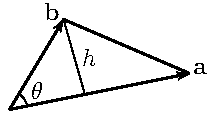
\includegraphics{sec_1_2_triangle.pdf}
\end{center}
}%
Thus the area of the triangle is  $\half|\va|\,|\vb|\,\sin\theta$.
By property 2 of the cross product in Theorem \eref{CLP200}{thm:crossPppties}
of the CLP-3 text,
 $|\va\times\vb|=|\va|\,|\vb|\,\sin\theta$. So
\begin{align*}
\text{area} &= \half|\va\times\vb|
=\half|\llt 1,2,3\rgt\times\llt 3,2,1\rgt| \\
&=\half | \hi\,(2-6)-\hj\,(1-9) +\hk\,(2-6)| \\
&=\half\sqrt{16+64+16} \\
&=2\sqrt{6} 
\end{align*}
\end{solution}

%%%%%%%%%%%%%%%%%%%%%%%%%%%%%%%%
\begin{question}[M200 2003D] %8
 A particle $P$ of unit mass whose position in space at time
$t$ is $\vr(t)$ has angular momentum $L(t)=\vr(t)\times\vr'(t)$.
If $\vr''(t)=\rho(t)\vr(t)$ for a scalar function $\rho$, show that
$L$ is constant, i.e. does not change with time. Here $'$ denotes 
$\diff{}{t}$.
\end{question}

\begin{hint}
Evaluate $\diff{L}{t}$ by differentiating $\vr(t)\times\vr'(t)$.
\end{hint}

\begin{answer}
See the solution.
\end{answer}

\begin{solution}
The derivative of $L$ is
\begin{align*}
\diff{L}{t}=\diff{}{t}\big(\vr(t)\times\vr'(t)\big)
=\vr'(t)\times\vr'(t)+\vr(t)\times\vr''(t)
=\vr'(t)\times\vr'(t)+\vr(t)\times\big(\rho(t)\vr(t)\big)
\end{align*}
Both terms vanish because the cross product of any two parallel vectors
is zero. So $\diff{L}{t}=0$ and $L(t)$ is independent of $t$. 
\end{solution}



%%%%%%%%%%%%%%%%%%
\subsection*{\Application}
%%%%%%%%%%%%%%%%%%

\begin{question}
Show that the diagonals of a parallelogram bisect each other.
\end{question}

%\begin{hint}
%\end{hint}

\begin{answer}
See the solution.
\end{answer}

\begin{solution}
The parallelogram determined by the vectors $\va$ and $\vb$
has vertices $\vZero,\ \va,\ \vb$ and $\va+\vb$.
As $t$ varies from $0$ to $1$, $t(\va+\vb)$ traverses the
diagonal from $\vZero$ to $\va+\vb$.
As $s$ varies from $0$ to $1$, $\va+s(\vb-\va)$ traverses the
diagonal from $\va$ to $\vb$. These two straight lines meet
when $s$ and $t$ are such that
\begin{equation*}
t(\va+\vb)=\va+s(\vb-\va)
\end{equation*}
or
\begin{equation*}
(t+s-1)\va=(s-t)\vb
\end{equation*}
Assuming that $\va$ and $\vb$ are not parallel (i.e. the parallelogram
has not degenerated to a line segment), this is the case only
when $t+s-1=0$ and $s-t=0$. That is, $s=t=\half$. So the two lines
meet at their midpoints.
\end{solution}

%%%%%%%%%%%%%%%%%%%%%%%%%%%%%%%%
\begin{question}
Consider a cube such that each side has length $s$. Name,
in order, the four vertices on the bottom of the cube $A, B, C, D$ and the
corresponding four vertices on the top of the cube $A', B', C', D'$.
\begin{enumerate}[(a)]
\item 
Show that all edges of the tetrahedron $A'C'BD$ have the same length.
\item
Let $E$ be the center of the cube. Find the angle between $EA$ and $EC$.
\end{enumerate}
\end{question}

%\begin{hint}
%
%\end{hint}

\begin{answer}
(a) All $6$ edges have length $\sqrt{2}s$.\qquad
(b) $109.5^\circ$
\end{answer}

\begin{solution}
We may choose our coordinate axes so that $A=(0,0,0)$,  $B=(s,0,0)$,
$C=(s,s,0)$, $D=(0,s,0)$ and $A'=(0,0,s)$, $B'=(s,0,s)$,
$C'=(s,s,s)$, $D'=(0,s,s)$.

(a) Then
\begin{alignat*}{5}
|A'C'|&=\big|\llt s,s,s\rgt -\llt 0,0,s\rgt \big|
      &&=\big|\llt s,s,0\rgt \big|&=\sqrt{2}\,s\\
|A'B|&=\big|\llt s,0,0\rgt -\llt 0,0,s\rgt \big|
     &&=\big|\llt s,0,-s\rgt \big|&=\sqrt{2}\,s\\
|A'D|&=\big|\llt 0,s,0\rgt -\llt 0,0,s\rgt \big|
     &&=\big|\llt 0,s,-s\rgt \big|&=\sqrt{2}\,s\\
|C'B|&=\big|\llt s,0,0\rgt -\llt s,s,s\rgt \big|
     &&=\big|\llt 0,-s,-s\rgt \big|&=\sqrt{2}\,s\\
|C'D|&=\big|\llt 0,s,0\rgt -\llt s,s,s\rgt \big|
     &&=\big|\llt -s,0,-s\rgt \big|&=\sqrt{2}\,s\\
|BD|&=\big|\llt 0,s,0\rgt -\llt s,0,0\rgt \big|
    &&=\big|\llt -s,s,0\rgt \big|&=\sqrt{2}\,s
\end{alignat*}

(b) $E=\half(s,s,s)$ so that $EA=\llt 0,0,0\rgt -\half\llt s,s,s\rgt 
      =-\half\llt s,s,s\rgt $ and 
$EC=\llt s,s,0\rgt -\half\llt s,s,s\rgt =\half\llt s,s,-s\rgt $.
$$
\cos\theta =\frac{-\llt s,s,s\rgt \cdot\llt s,s,-s\rgt}
                 {|\llt s,s,s\rgt |\,|\llt s,s,-s\rgt |}
        =\frac{-s^2}{3s^2}
        =-\frac{1}{3}
\qquad \implies\quad \theta=109.5^\circ
$$
\end{solution}

%%%%%%%%%%%%%%%%%%%%%%%%%%%%%%%%
\begin{question}
Find the angle between the diagonal of a cube and the diagonal
of one of its faces.
\end{question}

%\begin{hint}
%
%\end{hint}

\begin{answer}
$35.26^\circ$ or $90^\circ$ or $144.74^\circ$
\end{answer}

\begin{solution}
Suppose that the cube has height, length and width $s$.
We may choose our coordinate axes so that the vertices
of the cube are at $(0,0,0)$, $(s,0,0)$, $(0,s,0)$, $(0,0,s)$, 
$(s,s,0)$, $(0,s,s)$, $(s,0,s)$ and $(s,s,s)$. 

We'll start with a couple of examples. The diagonal from $(0,0,0)$
to $(s,s,s)$ is $\llt s,s,s\rgt$. One face of the cube has vertices $(0,0,0)$,
$(s,0,0)$, $(0,s,0)$ and $(s,s,0)$. One diagonal of this face runs from
$(0,0,0)$ to $(s,s,0)$ and hence is $\llt s,s,0\rgt$. The angle between 
$\llt s,s,s\rgt$ and $\llt s,s,0\rgt$ is
\begin{align*}
\cos^{-1}\left(\frac{\llt s,s,s\rgt\cdot\llt s,s,0\rgt}
                    {|\llt s,s,s\rgt|\,|\llt s,s,0\rgt|}\right)
=\cos^{-1}\left(\frac{2s^2}{\sqrt{3}s\,\sqrt{2}s}\right)
=\cos^{-1}\left(\frac{2}{\sqrt{6}}\right)\approx 35.26^\circ
\end{align*}
A second diagonal for the face with vertices  $(0,0,0)$,
$(s,0,0)$, $(0,s,0)$ and $(s,s,0)$ is that running from
$(s,0,0)$ to $(0,s,0)$. This diagonal is $\llt -s,s,0\rgt$. The angle between 
$\llt s,s,s\rgt$ and $\llt -s,s,0\rgt$ is
\begin{align*}
\cos^{-1}\left(\frac{\llt s,s,s\rgt\cdot\llt -s,s,0\rgt}
               {|\llt s,s,s\rgt|\,|\llt -s,s,0\rgt|}\right)
=\cos^{-1}\left(\frac{0}{\sqrt{3}s\,\sqrt{2}s}\right)
=\cos^{-1}(0)=90^\circ
\end{align*}

Now we'll consider the general case.
Note that every component of every vertex of the cube is either $0$ or
$s$. In general, two vertices of the cube are at
opposite ends of a diagonal of the cube if all three components of the
two vertices are different. For example, if one end of the diagonal is
$(s,0,s)$, the other end is $(0,s,0)$. The diagonals of the cube are all 
of the form $\llt \pm s,\pm s,\pm s\rgt$. All of these diagonals are of length $\sqrt{3}s$.
Two vertices are on the same face of the cube if one of their components
agree. They are on opposite ends of a diagonal for the face if their other
two components differ. For example $(0,s,s)$ and $(s,0,s)$ are both on
the face with $z=s$.  Because the $x$ components $0,\ s$ are different
and the $y$ components $s,\ 0$ are different, $(0,s,s)$ and $(s,0,s)$
are the ends of a diagonal of the face with $z=s$. The diagonals of the
faces with $z=0$ or $z=s$ are $\llt \pm s,\pm s,0\rgt$. The diagonals of the
faces with $y=0$ or $y=s$ are $\llt \pm s,0, \pm s\rgt$. The diagonals of the
faces with $x=0$ or $x=s$ are $\llt 0,\pm s,\pm s\rgt$. All of these diagonals
have length $\sqrt{2}s$. The dot product of one the cube diagonals
$\llt \pm s,\pm s,\pm s\rgt$ with one of the face diagonals  $\llt \pm s,\pm s,0\rgt$,
 $\llt \pm s,0, \pm s\rgt$, $\llt 0,\pm s,\pm s\rgt$ is of the form $\pm s^2\pm s^2+0$
and hence must be either $2s^2$ or $0$ or $-2s^2$. In general, the angle
between a cube diagonal and a face diagonal is
\begin{align*}
\cos^{-1}\left(\frac{\text{$2s^2$ or 0 or $-2s^2$}}{\sqrt{3}s\,\sqrt{2}s}\right)
=\cos^{-1}\left(\frac{\text{$2$ or $0$ or $-2$}}{\sqrt{6}}\right)\approx 
\text{$35.26^\circ$ or $90^\circ$ or $144.74^\circ$}. 
\end{align*}
\end{solution}


%%%%%%%%%%%%%%%%%%%%%%%%%%%%%%%%%%%%
\begin{question}
Consider a skier who is sliding without friction on the
hill $y=h(x)$ in a two dimensional world. The skier is subject to two
forces. One is gravity. The other acts perpendicularly to the hill. The second force automatically adjusts its magnitude so as to prevent the skier from burrowing into the hill. Suppose that the skier became
airborne at some $(x_0,y_0)$ with $y_0=h(x_0)$. How fast was the skier going? 

\end{question}

%\begin{hint}
%\end{hint}

\begin{answer}
$\sqrt{1+h'\big(x_0\big)^2}\sqrt{-g/h''\big(x_0\big)}$
\end{answer}

\begin{solution}
Denote by $\big(x(t),y(t)\big)$ the position of the skier at time $t$. As long as the skier remains on the surface of the hill
\begin{align*}
y(t)&=h\big(x(t)\big)   \\
\implies y'(t)&=h'\big(x(t)\big)\,x'(t)  \\
\implies y''(t)&=h''\big(x(t)\big)\, x'(t)^2+h'\big(x(t)\big)\,x''(t)
\end{align*}
So the velocity and acceleration vectors of the skier are
\begin{align*}
\vv(t)&=\llt 1,h'\big(x(t)\big)\rgt x'(t) \\
\va(t)&=\llt 1,h'\big(x(t)\big)\rgt x''(t)
+\llt 0,h''\big(x(t)\big)\rgt x'(t)^2
\end{align*}
The skier is subject to two forces. One is gravity. The other
acts perpendicularly to the hill and has a magnitude such that the skier
remains on the surface of the hill. From the velocity vector of the
skier (which remain tangential to the hill as long as the skier
remains of the surface of the hill),we see that one vector normal to
the hill at $\big(x(t),y(t)\big)$ is 
$$
\vn(t)=\llt-h'\big(x(t)\big),1\rgt
$$
This vector is not a unit  vector, but that's ok. By Newton's law
of motion
\begin{equation*}
m\va=-mg\,\hj+p(t)\,\vn(t)
\end{equation*}
for some function $p(t)$.
Dot both sides of this equation with $\vn(t)$.
\begin{equation*}
m\va(t)\cdot\vn(t)=-mg\hj\cdot\vn(t)+p(t)|\vn(t)|^2
\end{equation*}
Substituting in
\begin{align*}
mh''\big(x(t)\big)\,x'(t)^2&=-mg+p(t)\left[1+h'\big(x(t)\big)^2\right] \\
\implies p(t)\left[1+h'\big(x(t)\big)^2\right]
&=m\Big(g+h''\big(x(t)\big)\,x'(t)^2\Big)
\end{align*}
As long as $p(t)\ge 0$, the hill is pushing up in order to keep the skier
on the surface. When $p(t)$ becomes negative, the hill has to pull on the
skier in order to keep her on the surface. But the hill can't pull, 
so the skier becomes airborne instead. This happens when
\begin{equation*}
g+h''\big(x(t)\big)x'(t)^2=0
\end{equation*}
That is when $x'(t)=\sqrt{-g/h''\big(x(t)\big)}$. At this time $x(t)=x_0$, $y(t)=y_0$ and the speed of the skier is 
\begin{equation*}
\sqrt{x'(t)^2+y'(t)^2}
=\sqrt{1+h'\big(x_0\big)^2}\sqrt{-g/h''\big(x_0\big)}
\end{equation*}
\end{solution}


%%%%%%%%%%%%%%%%%%%%%%%%%%%%%%%%%%%%
\begin{question}
A marble is placed on the plane $ax+by+cz=d$. The coordinate
system has been chosen so that the positive $z$--axis points straight up.
The coefficient $c$ is nonzero and the coefficients $a$ and $b$ are not
both zero.
In which direction does the marble roll? 
Why were the conditions ``$c\ne 0$'' and ``$a,b$ not both zero'' imposed?
\end{question}

%\begin{hint}
%\end{hint}

\begin{answer}
The marble rolls in the directionn$\llt ac,bc,-a^2-b^2\rgt$.
If $c=0$, the plane is vertical. In this case, the marble
doesn't roll -- it falls straight down. If $a=b=0$, the plane is horizontal.
 In this case, the marble doesn't roll --- it remains stationary.
\end{answer}

\begin{solution}
The marble is subject to two forces. The first, gravity, is
$-mg\,\hk$ with $m$ being the mass of the marble. The second is the normal
force imposed by the plane. This forces acts in a direction perpendicular
to the plane. One vector normal to the plane is $a\,\hi+b\,\hj+c\,\hk$. 
So the force due to the plane is $T\llt a,b,c\rgt$ with $T$ determined  by the
property that the net force perpendicular to the plane must be exactly
zero, so that the marble remains on the plane, neither digging into nor
flying off of it. The projection of the gravitational force onto the normal
vector $\llt a,b,c\rgt$ is
\begin{equation*}
\frac{-mg\llt 0,0,1\rgt\cdot\llt a,b,c\rgt}{|\llt a,b,c\rgt|^2}\llt a,b,c\rgt
=\frac{-mgc}{a^2+b^2+c^2}\llt a,b,c\rgt
\end{equation*}
The condition that determines $T$ is thus
\begin{equation*}
T\llt a,b,c\rgt+\frac{-mgc}{a^2+b^2+c^2}\llt a,b,c\rgt =0
\implies T=\frac{mgc}{a^2+b^2+c^2}
\end{equation*}
The total force on the marble is then (ignoring friction -- which will
have no effect on the direction of motion)
\begin{align*}
T\llt a,b,c\rgt-mg\llt 0,0,1\rgt&=\frac{mgc}{a^2+b^2+c^2}\llt a,b,c\rgt-mg\llt 0,0,1\rgt\cr
&=mg\frac{c\llt a,b,c\rgt-\llt 0,0,a^2+b^2+c^2\rgt}{a^2+b^2+c^2}\cr
&=mg\frac{\llt ac,bc,-a^2-b^2\rgt}{a^2+b^2+c^2}\cr
\end{align*}
The direction of motion $\llt ac,bc,-a^2-b^2\rgt$. If you want to turn
this into a unit vector, just divide by $\sqrt{(a^2+b^2)(a^2+b^2+c^2)}$.
Note that the direction vector in perpendicular $\llt a,b,c\rgt$ and hence is parallel
to the plane. If $c=0$, the plane is vertical. In this case, the marble
doesn't roll -- it falls straight down. If $a=b=0$, the plane is horizontal.
 In this case, the marble doesn't roll --- it remains stationary.
\end{solution}

%%%%%%%%%%%%%%%%%%%%%%%%%%%%%%%%%%%%
\begin{question}
Show that $\va\cdot(\vb\times\vc)
                         =(\va\times\vb)\cdot\vc$.
\end{question}

%\begin{hint}
%\end{hint}

\begin{answer}
See the solution.
\end{answer}

\begin{solution} By definition, the left and right hand sides are
\begin{align}
\va\cdot(\vb\times\vc)
&=\llt a_1,a_2,a_3\rgt \cdot\llt b_2c_3-b_3c_2, b_3c_1-b_1c_3, b_1c_2-b_2c_1\rgt \notag\\
&=a_1b_2c_3 - a_1b_3c_2 + a_2b_3c_1 - a_2b_1c_3 + a_3b_1c_2 - a_3b_2c_1
\tag{lhs}\\
\notag\\
(\va\times\vb)\cdot\vc
&=\llt a_2b_3-a_3b_2, a_3b_1-a_1b_3, a_1b_2-a_2b_1\rgt \cdot\llt c_1,c_2,c_3\rgt \notag\\
&=a_2b_3c_1 - a_3b_2c_1 + a_3b_1c_2 - a_1b_3c_2 + a_1b_2c_3 - a_2b_1c_3
\tag{rhs}
\end{align}
(lhs) and (rhs) are the same.
\end{solution}


%%%%%%%%%%%%%%%%%%%%%%%%%%%%%%%%%%%%
\begin{question}
Show that $\va\times(\vb\times\vc)
=(\va\cdot\vc)\vb-(\va\cdot\vb)\vc$.
\end{question}

%\begin{hint}
%\end{hint}

\begin{answer}
See the solution.
\end{answer}

\begin{solution}
By definition, 
\begin{align*}
\vb\times\vc
\ =\ &(b_2c_3-b_3c_2)\hi-(b_1c_3-b_3c_1)\hj
    +(b_1c_2-b_2c_1)\hk \\
\intertext{so that the left and right hand sides are}
\va\times(\vb\times\vc)
\ =\ &\det\left[\begin{matrix}\hi&\hj &\hk\\
                     a_1&a_2&a_3\\
            b_2c_3-b_3c_2&-b_1c_3+b_3c_1&b_1c_2-b_2c_1\end{matrix}\right]\\
\ =\ &\hi\,[a_2(b_1c_2-b_2c_1)-a_3(-b_1c_3+b_3c_1)]\\
{-}&\hj\,[a_1(b_1c_2-b_2c_1)-a_3(b_2c_3-b_3c_2)]\\
{+}&\hk\,[a_1(-b_1c_3+b_3c_1)-a_2(b_2c_3-b_3c_2)]&{\rm (lhs)}\\
\noalign{\vskip0.05in}
(\va\cdot\vc)\vb-(\va\cdot\vb)\vc
\ =\ &(a_1c_1+a_2c_2+a_3c_3)(b_1\hi+b_2\hj+b_3\hk)
-(a_1b_1+a_2b_2+a_3b_3)(c_1\hi+c_2\hj+c_3\hk)\\
{=}\ &
\hi\,[a_1b_1c_1+a_2b_1c_2+a_3b_1c_3-a_1b_1c_1-a_2b_2c_1-a_3b_3c_1]
\\
{+}&\hj\,[a_1b_2c_1+a_2b_2c_2+a_3b_2c_3-a_1b_1c_2-a_2b_2c_2-a_3b_3c_2]
\\
{+}&\hk\,[a_1b_3c_1+a_2b_3c_2+a_3b_3c_3-a_1b_1c_3-a_2b_2c_3-a_3b_3c_3]\cr
{=}\ &
\hi\,[a_2b_1c_2+a_3b_1c_3-a_2b_2c_1-a_3b_3c_1]
\\
{+}&\hj\,[a_1b_2c_1+a_3b_2c_3-a_1b_1c_2-a_3b_3c_2]
\\
{+}&\hk\,[a_1b_3c_1+a_2b_3c_2-a_1b_1c_3-a_2b_2c_3]
&{\rm (rhs)}
\end{align*}
(lhs) and (rhs) are the same.
\end{solution}


%%%%%%%%%%%%%%%%%%%%%%%%%%%%%%%%%%%%
\begin{question}
Derive a formula for $(\va\times\vb)\cdot(\vc\times\vd)$
that involves dot but not cross products.
\end{question}

%\begin{hint}
%\end{hint}

\begin{answer}
$(\va\times\vb)\cdot(\vc\times\vd)=
(\va\cdot\vc)(\vb\cdot\vd)
-(\va\cdot\vd)(\vb\cdot\vc)$
\end{answer}

\begin{solution}
By properties 9 and 10 of Theorem \eref{CLP200}{thm:crossPppties} in the CLP-3 
text,
\begin{align*}
(\va\times\vb)\cdot(\vc\times\vd)
&=\va\cdot[\vb\times(\vc\times\vd)]
\hskip.5in&\text{(by property 9 with $\vc\rightarrow (\vc\times\vd)$)} \\
&=\va\cdot[(\vb\cdot\vd)\vc-(\vb\cdot\vc)\vd]
\hskip.25in&\text{(by property 10)}\cr
&=(\va\cdot\vc)(\vb\cdot\vd)
-(\va\cdot\vd)(\vb\cdot\vc)
\end{align*}
So
\begin{equation*}
(\va\times\vb)\cdot(\vc\times\vd)=
(\va\cdot\vc)(\vb\cdot\vd)
-(\va\cdot\vd)(\vb\cdot\vc)
\end{equation*}
\end{solution}


%%%%%%%%%%%%%%%%%%%%%%%%%%%%%%%%%%%%
\begin{question}
A prism has the six vertices
\begin{alignat*}{3}
A&=(1,0,0)\qquad   &  A'&=(5,0,1) \\
B&=(0,3,0)   &  B'&=(4,3,1) \\
C&=(0,0,4)   &  C'&=(4,0,5) 
\end{alignat*}
\begin{enumerate}[(a)]
\item
  Verify that three of the faces are parallelograms.
  Are they rectangular?
\item
  Find the length of $AA'$.
\item
  Find the area of the triangle $ABC$.
\item
   Find the volume of the prism.
\end{enumerate}
\end{question}

%\begin{hint}
%\end{hint}

\begin{answer}
(a)
$AA'B'B$ is a parallelogram, but not a rectangle.\\
$AA'C'C$ is a rectangle.\\
$BB'C'C$ is a parallelogram, but not a rectangle.

(b) $\sqrt{17}$ \qquad
(c) $\frac{13}{2}$\qquad
(d) $\frac{51}{2}$


\end{answer}

\begin{solution}
(a) $AA'=\llt 4,0,1\rgt $ and $BB'=\llt 4,0,1\rgt $ are opposite sides
of the quadrilateral $AA'B'B$. They have the same length 
and direction. The same is true for $AB=\llt -1,3,0\rgt $ and 
$A'B'=\llt -1,3,0\rgt $. So $AA'B'B$ is a parallelogram. Because, 
$AA'\cdot AB=\llt 4,0,1\rgt \cdot\llt -1,3,0\rgt =-4\ne 0$, 
the neighbouring edges of $AA'B'B$ are not perpendicular and so $AA'B'B$ 
is \emph{not} a rectangle.

Similarly, the quadilateral $ACC'A'$ has opposing sides
$AA'=\llt 4,0,1\rgt =CC'=\llt 4,0,1\rgt $ and 
$AC=\llt -1,0,4\rgt =A'C'=\llt -1,0,4\rgt $ and so is
a parallelogram. Because $AA'\cdot AC=\llt 4,0,1\rgt \cdot\llt -1,0,4\rgt = 0$, the neighbouring edges of $ACC'A'$ are perpendicular, so
$ACC'A'$ \emph{is} a rectangle.

Finally, the quadilateral $BCC'B'$ has opposing sides
$BB'=\llt 4,0,1\rgt =CC'=\llt 4,0,1\rgt $ and 
$BC=\llt 0,-3,4\rgt =B'C'=\llt 0,-3,4\rgt $ and so is
a parallelogram. Because $BB'\cdot BC=\llt 4,0,1\rgt \cdot\llt 0,-3,4\rgt 
= 4\ne 0$, the neighbouring edges of $BCC'B'$ are not perpendicular, so 
$BCC'B'$ is \emph{not} a rectangle.

(b) The length of $AA'$ is $|\llt 4,0,1\rgt |=\sqrt{16+1}=\sqrt{17}$.

(c) The area of a triangle is one half its base times its height. 
That is, one half times $|AB|$ times $|AC|\sin\theta$, where 
$\theta$ is the angle between $AB$ and $AC$. This is precisely 
$\half |AB\times AC|=\half|\llt -1,3,0\rgt \times\llt -1,0,4\rgt | 
=\half |\llt 12,4,3\rgt|=\frac{13}{2}$.

(d) The volume of the prism is the area of its base $ABC$,
 times its height, which is the length of $AA'$ times the cosine of the
angle between $AA'$ and the normal to $ABC$. This coincides with
$\half \llt 12,4,3\rgt \cdot\llt 4,0,1\rgt =\half(48+3)=\frac{51}{2}$, which is 
one half times the length of $\llt 12,4,3\rgt $ (the area of $ABC$) 
times the length of $\llt 4,0,1\rgt $ (the length of $AA'$) times the 
cosine of the angle between $\llt 12,4,3\rgt $ and
$\llt 4,0,1\rgt $ (the angle between the normal to $ABC$ and $AA'$).

\end{solution}

%%%%%%%%%%%%%%%%%%%%%%%%%%%%%%%%%%%%
\begin{question}\label{prb pythagorous}
(Three dimensional Pythagorean Theorem) A solid body in space 
with exactly four vertices is called a tetrahedron. Let $A$, $B$, $C$ and
$D$ be the areas of the four faces of a tetrahedron. Suppose that the
three edges meeting at the vertex opposite the face of area $D$ are 
perpendicular to each other. Show that $D^2=A^2+B^2+C^2$.

\begin{center}
     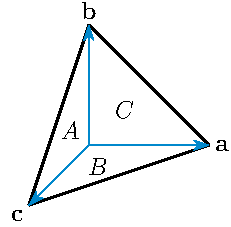
\includegraphics{tetrahedron.pdf}
\end{center}

\end{question}

\begin{hint}
Choose coordinate axes so that the vertex opposite
the face of area $D$ is at the origin. Denote  by $\va$, $\vb$ and
$\vc$ the vertices opposite the sides of area $A$, $B$ and $C$ respectively.
Express $A$, $B$, $C$ and $D$, which are areas of triangles, as one half 
times cross products of vectors built from $\va$, $\vb$ and $\vc$.
\end{hint}

\begin{answer}
See the solution.
\end{answer}

\begin{solution}
Choose our coordinate axes so that the vertex opposite
the face of area $D$ is at the origin. Denote  by $\va$, $\vb$ and
$\vc$ the vertices opposite the sides of area $A$, $B$ and $C$ respectively.
Then the face of area $A$ has edges $\vb$ and $\vc$ so that
$A=\half |\vb\times\vc|$. Similarly $B=\half|\vc\times\va|$ and
$C=\half|\va\times \vb|$. The face of area $D$ is the triangle 
spanned by $\vb-\va$ and $\vc-\va$ so that
\begin{align*}
D&=\half|(\vb-\va)\times(\vc-\va)|\cr
&=\half|\vb\times \vc-\va\times\vc-\vb\times\va|\\
&=\half|\vb\times \vc+\vc\times\va+\va\times\vb|
\end{align*} 
By hypothesis, the vectors $\va$, $\vb$ and $\vc$ are all perpendicular
to each other. Consequently the vectors $\vb\times \vc$ (which is
a scalar times $\va$), $\vc\times\va$ (which is a scalar times
$\vb$) and $\va\times\vb$ (which is a scalar times $\vc$)
are also mutually perpendicular. So, when we multiply out
\begin{equation*}
D^2=\frac{1}{4}\big[\vb\times \vc+\vc\times\va+\va\times\vb\big]\cdot\big[\vb\times \vc+\vc\times\va+\va\times\vb\big]
\end{equation*}
all the cross terms vanish, leaving
\begin{equation*}
D^2=\frac{1}{4}\big[(\vb\times \vc)\cdot(\vb\times \vc)
+(\vc\times\va)\cdot(\vc\times\va)
+(\va\times\vb)\cdot(\va\times\vb)\big]=A^2+B^2+C^2
\end{equation*}
\end{solution}

%%%%%%%%%%%%%%%%%%%%%%%%%%%%%%%%%%%%
\begin{question}
(Three dimensional law of cosines)  Let $A$, $B$, $C$ and
$D$ be the areas of the four faces of a tetrahedron. Let 
$\al$ be the angle between the faces with areas $B$ and $C$, 
$\be$ be the angle between the faces with areas $A$ and $C$ and 
$\ga$ be the angle between the faces with areas $A$ and $B$. 
(By definition, the angle between two faces is the angle between the normal vectors to the faces.)
 Show that 
\begin{equation*}
D^2=A^2+B^2+C^2-2BC\cos\al-2AC\cos\be-2AB\cos\ga
\end{equation*}
\end{question}

\begin{hint}
  Do problem \ref{prb pythagorous} first.
\end{hint}

\begin{answer}
See the solution.
\end{answer}

\begin{solution}
As in problem \ref{prb pythagorous},
\begin{equation*}
D^2=\frac{1}{4}
  \big[\vb\times \vc+\vc\times\va+\va\times\vb\big]\cdot
  \big[\vb\times \vc+\vc\times\va+\va\times\vb\big]
\end{equation*}
But now $(\vb\times \vc)\cdot(\va\times\vc)$, instead of vanishing,
is $|\vb\times \vc|=2A$ times $|\va\times\vc|=2B$ times
the cosine of the angle between $\vb\times \vc$ (which is perpendicular
to the face of area $A$) and $\va\times\vc$ (which is perpendicular
to the face of area $B$). That is
\begin{align*}
(\vb\times \vc)\cdot(\va\times\vc)&=4 AB\cos \ga\\
(\va\times \vb)\cdot(\vc\times\vb)&=4 AC\cos \be\\
(\vb\times \va)\cdot(\vc\times\va)&=4 BC\cos \al
\end{align*}
(If you're worried about the signs, that is, if you are worried about 
why $(\vb\times \vc)\cdot(\va\times\vc)=4 AB\cos \ga$
rather than $(\vb\times \vc)\cdot(\vc\times\va)=4 AB\cos \ga$,
note  that when $\va\approx\vb$, 
$(\vb\times \vc)\cdot(\va\times\vc)\approx|\vb\times\vc|^2$ is positive and 
$(\vb\times \vc)\cdot(\vc\times\va) \approx -|\vb\times\vc|^2$ is negative.) Now, expanding out
\begin{align*}
D^2\ =\ &\frac{1}{4}
   \big[\vb\times \vc+\vc\times\va+\va\times\vb\big]\cdot
   \big[\vb\times \vc+\vc\times\va+\va\times\vb\big] \\
=\ &\frac{1}{4}\big[(\vb\times \vc)\cdot(\vb\times \vc)
     +(\vc\times\va)\cdot(\vc\times\va)
     +(\va\times\vb)\cdot(\va\times\vb) \\
&+2(\vb\times \vc)\cdot(\vc\times \va)
 +2(\vb\times \vc)\cdot(\va\times \vb)
 +2(\vc\times \va)\cdot(\va\times \vb)\big] \\
=\ &A^2+B^2+C^2-2 AB\cos \ga-2 AC\cos \be-2 BC\cos \al
\end{align*}
\end{solution}




